% ----------------------------------------------------------------------------
% Copyright (c) 2016 by Burkhardt Renz. All rights reserved.
% Die Vorlage für eine Abschlussarbeit in der Informatik am Fachbereich
% MNI der THM ist lizenziert unter einer Creative Commons
% Namensnennung-Nicht kommerziell 4.0 International Lizenz.
%
% Id:$
% ----------------------------------------------------------------------------
\chapter{Implementierung}
\label{chapter:Implementierung}

In diesem Kapitel werden Implementierungen von Prototypen gezeigt, die im Kapitel \cref{chapter:Design} besprochen sind. In \cref{section:Instrumentalisierungsbibliothek: Traktor} werden die Implementierungsdetails der Instrumentalisierungsbilbiothek \textbf{Traktor} vorgestellt. In \cref{section:Traktor Agent} und in \cref{section:Traktor Registry} werden die Traktor Services beschrieben. Anschließend werden zwei Anwendungsfälle gezeigt. Der Anwendungsfall des Rendering-System in \cref{section:Unity Rendering System} und der Anwendungsfall einer verteilten Webanwendung in \cref{section:Webserver Entwicklungsumgebung}

\section{Instrumentalisierungsbibliothek: Traktor}
\label{section:Instrumentalisierungsbibliothek: Traktor}
In diesem Kapitel wird die Implementierung der Instrumentalisierungsbibliothek Traktor vorgestellt. Es wird das Datenmodell umgesetzt, welches in \cref{section:Datenmodell} konzipiert ist und gezeigt, inwiefern Traktor die Anforderungen erfüllt.

Traktor ist eine Instrumentalisierungsbibliothek, die sich die OpenTracing API als Vorbild nimmt. Die OpenTracing API ist eine herstellerneutrale Instrumentalisierungs-API, die unter der Schirmherschafft der \gls{cncfLabel} steht, welches Teil der gemeinnützig agierenden \gls{lfLabel} ist.

Die zwei zentralen Einheiten der Traktor Instrumentalisierungsbibliothek sind der in \cref{subsection:Tracer} gezeigte \textbf{Tracer} und die in \cref{subsection:Span} gezeigten \textbf{Spans}. Weitere Klassen, die den in \cref{subsection:Tracingcontext innerhalb eines Systems} beschriebenen Designansatz implementieren, sind der in \cref{subsection:Scope} vorgestellte \textbf{Scope} und der in \cref{subsection:ScopeManager} vorgestellte \textbf{ScopeManager}. Die Kontextpropagierung, die mit einer Websocketverbindung innerhalb des Tracer und der, in \cref{section:Traktor Registry} gezeigten,\textbf{ Traktor Registry}, umgesetzt ist, implementiert den in \cref{subsection:Tracingcontext über Systemgrenzen} erläuterten Designansatz. Ein Gesamtüberblick mit allen Relationen der Klassen, wird in \cref{subsection:UML-Klassendiagramm der Bibliothek} gegeben.

\subsection{Tracer}
\label{subsection:Tracer}
Der Tracer ist die zentrale Verwaltungseinheit der Instrumentalisierung. Dieser verwaltet die Verbindung der Anwendungsinstrumentalisierung zu dem Agenten und der Registry. Der Tracer kümmert sich um das Generieren von Spans und die Herstellung von Kausalzusammenhängen zwischen den Spans. Außerdem stellt der Tracer die Funktionalitäten zur Kontextpropagierung über die Registry bereit. Die Spans sind Darstellungen von ausgeführter Arbeit in einer instrumentalisierten Anwendung. 

Die Tracer API erweitert die OpenTracing API um vier Funktionen, die notwendig sind, um sich mit der Tracinginfrastuktur zu verbinden. Die \emph{Configure} Funktion sorgt für einen Verbindungsaufbau, abhängig von den übergebenen Parametern. Ein vollständiger Verbindungsaufbau ist nötig, um eine Kontextpropagierung zu ermöglichen. Außerdem wird der \gls{udpLabel}-Klient initialisiert, damit beendete Spans reportet werden können. Der \gls{udpLabel}-Klient hat einen Port zu belegen, der angegeben werden muss. Die IP-Adressen der Services sind dem Tracer bekannt zu geben. Auch der Port auf der die Anwendung lauscht, muss übergeben werden. Die Configure Funktion verwendet die \emph{Register} Funktion zur Erstellung einer \textbf{WebSocketClient} Instanz. Die Websocketverbindung wird über die Lebensdauer des Tracer offen gehalten. Über diesen Kommunikationskanal werden die Kontextinformationen übermittelt. \cref{listing:Tracer Verbindungsaufbau} zeigt eine Beispielhafte Konfigurierung. Dabei wird eine Tracerinstanz instanziiert und mit den Adressen der Traktorservices konfiguriert.

\begin{minipage}[]{\textwidth}
	\begin{lstlisting}[frame=trBL]
	using Traktor;
	
	var registryAddress = "localhost";
	var registryPort = "8080";
	var agentAddress = "localhost"
	var agentPort = 13337;
	var reporterPort = 13338;
	
	Tracer tracer = new Tracer();
	tracer.Configure(registryAddress,registryPort,agentAddress,
				agentPort,reporterPort);
	
	\end{lstlisting}
	\captionof{lstlisting}{Tracer Verbindungsaufbau mit der Registry und dem Reporter }
	\label{listing:Tracer Verbindungsaufbau}
\end{minipage} 

Die Kontextdaten werden in einer \emph{Carrier} Instanz gespeichert und über die Leitung gesendet. In der Implementierung gibt es genau einen Carriertyp. Der BinaryCarrier ist ein Datencontainer, der die Kontextinformationen als MemoryStream speichert. Der MemoryStream speichert die Daten im Arbeitsspeicher als Bytearray. Das Format wurde für die Übertragung über eine \gls{tcpLabel}/\gls{ipLabel} Verbindung ausgewählt, da die Kontextpropagierung über das Websocketprotokoll realisiert wird. Das Websocketprotokoll ist ein auf dem \gls{tcpLabel} basierendes Protokoll.
Die Spangenerierung wird durch eine \emph{SpanBuilder} Instanz geregelt. Der Operationsname wird der SpanBuilder Instanz mitgegeben und für die Generierung des Spans genutzt. Die Kontextpropagierung wird durch die beiden sich ergänzenden asynchronen Funktionen \emph{SendContext} und \emph{ReceiveContext} implementiert. Dabei werden die Funktionen \emph{Extract} und \emph{Inject} verwendet. Die Inject Funktion erstellt einen BinaryCarrier, der für die Kontextübertragung genutzt wird. Die Extract Funktion extrahiert die Daten aus dem BinaryCarrier.

Der Tracer hält eine \textbf{Scopemanager} Instanz. Der Scopemanager verwaltet die Spans. Über den Scopemanager kann der Tracer den aktuell aktiven Span ermitteln.


\subsection{Span}
\label{subsection:Span}
Der Span beinhaltet alle relevanten Daten, die für das Repäsentieren eines Events in einem System notwendig sind. Darunter zählt ein Operationsname. Der Operationsname kann beispielsweise die Sematik des Events beschreiben. Auch bietet sich ein Funktionsname innerhalb der Anwendung an, falls der Span genau diesen umfasst. Der \textbf{Startzeitstempel} und der \textbf{Endzeitstempel} beschreibt die Zeitspanne, in der das Event stattfindet. Diese sind in der Implementierung \emph{Datetime}-Instanzen. Das Datetimeformat, welches für die Tracinginfrastruktur genutzt wird, hat folgenden Aufbau:

\begin{minipage}[]{\textwidth}
	\begin{lstlisting}[frame=trBL]
	MM/dd/yyyy hh:mm:ss.ffff tt
	\end{lstlisting}
	\captionof{lstlisting}{Zeitstempelformat der Spans}
	\label{listing:Tracer Verbindungsaufbau}
\end{minipage} 

Der Aufbau orientiert sich an dem amerikanischen Zeitformat. \textbf{MM} steht für den Monat, \textbf{dd} für den Tag und \textbf{yyyy} für das Jahr. Interessanter wird es bei dem Tageszeitformat. In einem System, bei dem Zeit eine kritische Rolle spielt, sind kleinste Zeitunterschiede von Bedeutung. \textbf{hh} und \textbf{mm} sind entsprechend die Stunden und Minunten. \textbf{ss.ffff} entspricht den Sekunden und dem Tausendstel einer Sekunde. \textbf{tt} steht für a.m beziehungsweise p.m., also der entsprechenden Tageshälfte der 2-mal-12-Stunden-Zählung. Die \textbf{Systemuhr Auflösung} ist an dieser Stelle erwähnenswert. Die Auflösung einer Uhr beschreibt die kleinste Einheit von Zeit, die akkurat von einer Uhr gemessen werden kann. Die Auflösung der Systemuhr hängt von dem Betriebssystem ab. In einem Windows 8  Betriebssystem ist die Standardresolution bei 15.6 ms. Das .NET Framework, welches für die Implementierung genutzt wird, behandelt verschiedene genutzte Softwaretimer wiederum eigenständig. Diese kann manuell auf 0.5 reduziert werden. In einem Linux-basierenden Betriebssystem hängt die Auflösung von der Software Clock ab. Dabei wird die Zeit in sog. \textbf{Jiffies} gemessen. Die Linux-Kernel version 2.6.0 führt eine jiffiegröße von 0.001 sekunden ein\footpartcite{mantime}. In dem verwendeten Windows 10 Betriebssystem ist die Standardauflösung der Systemuhr bei 1ms. Diese Auflösung ist für die Zeitmessung zufriedenstellend. Dem entsprechen sind die gemessenen Zeitstempel mit diesen Hintergrundinformationen zu bewerten. Eine höhere Auflösung ist in dem jeweiligen Betriebssystem durch die Verwendung eines \emph{Performance Counters} erzielbar. Unter Windows kann der \emph{QueryPerformanceCounter} genutzt werden, um einen Nanosekunden genauen Zeitstempel zu erhalten. Unter Linux kann die Betriebssystemfunktion \emph{clock\_gettime} genutzt werden, um einen Nanosekunden genauen Zeitstempel zu erhalten.

Ein Span besitzt einen Spankontext und eine Referenzliste. Der Inhalt des Spankontext wird in \cref{subsection:SpanContext} beschrieben. Die Referenzliste beinhaltet alle Spans, die eine \textbf{Happens-Before Relation} zu dem Span aufweisen. Das bedeutet, dass alle Elternspans, beispielsweise aus \emph{Child-Of} und \emph{Follows-From} resultierenden Beziehungen, in dieser Liste referenziert werden.

Schlussendlich kennt ein Span seinen Tracer, indem das Spanobjekt eine Referenz zu dem Tracerobjekt hält. Dies ist erforderlich, da beim fertigstellen des Spans die \emph{Finish} Funktion aufgerufen wird. Diese sorgt dafür, dass der Endzeitstempel gesetzt wird. Ausserdem wird die \emph{Report} Funktion der Reporterinstanz, bekannt durch den Tracer, aufgerufen. 

\subsection{SpanBuilder}
\label{subsection:SpanBuilder}

Der SpanBuilder ist das Bindeglied zwischen dem Tracer und der Spangenerierung. Der Anwender der Instrumentalisierungsbibliothek kann durch die \emph{BuildSpan} Funktion des Tracer die Spangenerierung einleiten. Dabei wird eine SpanBuilder Instanz erstellt, die die übergebenen Parameter zur Spangenerierung nutzt. Der SpanBuilder verlang, während der Initialisierung, nach einem Operationsnamen und der Referenz des aufrufenden Tracers. Diese werden als Felder in der SpanBuilder Instanz gespeichert. Durch die Funktionen \emph{AddReference} und \emph{AsChildOf} kann das Feld \emph{references} bearbeitet werden. Dabei ist AsChildOf eine spezialisierte Form der AddReference Funktion. Die AddReference Funktion erwartet einen Referenztypen und einen SpanContext als Paramenter. Diese werden dann für den zu bauenden Span genutzt. 

Eine weitere Grundfunktion ist die \emph{Start} Funktion. Diese beinhaltet die nötige Anwendungslogik, für die Traceidentifikationsnummergenerierung. Auch die Spanidentifikationsnummer wird generiert. Anschließend wird der Span gebaut und mit den gesammelten Daten initialisiert.

Ähnlich wie bei der AddReference Funktion, ist die \emph{StartActive} Funktion eine Spezialisierungen der Start Funktion. Die überladene StartActive Funktion kann parameterlos oder mit dem Boolean \emph{finishSpanOnDispose} aufgerufen werden. Der Boolean bestimmt, wie mit einem Span umgegangen wird, nachdem die entsprechende Finish Funktion aufgerufen worden ist. StartActive setzt den gebauten Span auf den Zustand \textbf{Aktiv}. Das bedeutet, dass der Scopemanager diesen verfolgt und gegebenfalls den vorherig aktiven Span zwischenspeichert.

Eine beispielhafte Nutzung des Spanbuilders sieht folgendermaßen aus:

\begin{minipage}[]{\textwidth}
	\begin{lstlisting}[frame=trBL]
	var operationname = "example_function";
	var spanBuilder = tracer.BuildSpan(operationname);
	var span = spanBuilder.Start();
	\end{lstlisting}
	\captionof{lstlisting}{Beispielhafte Anwendung des SpanBuilder}
	\label{listing:SpanBuiler}
\end{minipage} 

Ein Operationsname wird definiert und als Paramenter für die BuildSpan Funktion genutzt. Anschließend wird durch die Start Funktion der SpanBuilder Instanz ein Span auf den Zustand Aktiv gesetzt.


\subsection{SpanContext}
\label{subsection:SpanContext}

Die SpanContext Klasse beinhaltet eine TraceId, eine SpanId und einen Rerenztypen als Felder. Diese werden bei der Initialisierung gesetzt. Die SpanContext-Klasse ist ein reine Datenkapselung. Semantisch sind die in der SpanContext enthaltenen Daten jene, die in einem BinaryCarrier, codiert als Bytearray, über die Leitung gesendet werden.

Ein Auszug eines Spankontexts aus dem Entwicklungssystem zeigt den Aufbau. Der Auszug stammt aus dem Registryservice. In dem Service wird der Nachricht auf die Konsole ausgebenen, sobald eine Propagierung ausgelöst worden ist.

\begin{minipage}[]{\textwidth}
	\begin{lstlisting}[frame=trBL]
	traktor-registry_1 | Client-Message: WIoJiNwldhLM;ZtDdH4lQ1a1b;child_of
	\end{lstlisting}
	\captionof{lstlisting}{Ein über die Registry propagierter Spankontext}
	\label{listing:SpanContext-Registry}
\end{minipage} 

Der Spankontext beinhaltet drei Daten. Eine TraceId, eine SpanId und einen Relationstyp.

\subsection{Scope}
\label{subsection:Scope}

Ein Scope ist ein lokaler Kontext, welcher von dem ScopeManager verwaltet wird. In einem Scope werden Spans verwaltet. Dadurch wird das in \cref{subsection:Tracingcontext innerhalb eines Systems} beschriebene Problem der Kontextverfolgbarkeit innerhalb eines Systems gelöst. Ein Scope wird in einem Prozess geführt. Während eines Kontextwechsel wird der aktive Span in einer Variable gespeicher und anschließend wird der aktive Span mit dem zu aktivierenden Span ersetzt. Dadurch ist bei einer Beendigung des aktiven Spans der vorherige Span wiederherstellbar. Traktor nutzt die AsyncLocalScope CSharp Implementierung des OpenTracing-Projekts.

\subsection{ScopeManager}
\label{subsection:ScopeManager}
Ein ScopeManager verwaltet Scopes. Bei einem Kontextwechsel, zum Beispiel bei einer Multi-Thread Implementierung, werden die Scopes durch den Manager verfolgt. Ein Scope ist nur innerhalb seines Prozesses relevant und beinhaltet einen aktiven Span. Über den Spanmanager lässt sich der Span, welcher durch einen aktiven Scope umfasst wird, ermitteln. Der Tracer ist dadurch jederzeit in der Lage, den aktiven Span und seinen Kontext zu nutzen. Wie auch der Scope, wird die ScopeManager Implementierung des OpenTracing-Projekts genutzt. 

\subsection{Reporter}
\label{subsection:Reporter}
Die Reporter Klasse kapselt die \gls{udpLabel}-Verbindung des Tracers zu dem Agentenservice. Dabei wird die Netzwerkddresse, sowie der Port gespeichert. Bei der Initialisierung des Reporters, wird die Verbindung mit den gegebenen Parametern hergestellt.

Die Reporter Klasse umfasst drei Funktionen. Die Funktion \emph{Connect} stellt mit gegebenen Parametern die Verbindung zu dem \gls{udpLabel}-Service her. Der \gls{udpLabel}-Klient wird als Feld gespeichert und kann zur weiteren Datenübertragung genutzt werden. Die Funktion \emph{Report} sendet eine kodierte Form des Spans zu dem Agentenservice. Die Kodierung wird durch die Funktion \emph{BuildMessage} implementiert. Traktor nutzt eine UTF-8 Kodierung für den Nachrichtenaustausch.

\subsection{UML-Klassendiagramm der Bibliothek}
\label{subsection:UML-Klassendiagramm der Bibliothek}

Die Instrumentalisierungsbibliothek ist in der Programmiersprache C\# implementiert. Ein Grund dafür ist, dass das verteilte Rendering-System relevante Komponenten in C\# implementiert und in diesen die Bibliothek genutzt werden soll. Die Programmiersprache eignet sich außerdem für die Entwicklung von Systemkomponenten, die in einer verteilten System zum Einsatz kommen, wie aus der Spezifikation der Programmiersprache entnommen werden kann: 

\begin{quote}
	\cbstart
	C\# ist gedacht als simple, moderne,  universal einsetzbare, objektorientierte Programmiersprache. [...] Die Sprache ist für die Entwicklung von Softwarekomponenten gedacht, die in einer verteilten Umgebung bereitgestellt werden.\footpartcite[S. xx]{10.5555/861332}
	\cbend
\end{quote}

Das Klassendiagramm, gezeigt in \cref{fig:TraktorKlassendiagramm}, stellt einen Überblick über die vorherig beschriebenen relevanten Entitäten der Bibliothek dar.

\newpage
\begin{landscape}
	\begin{figure}
		\centering
		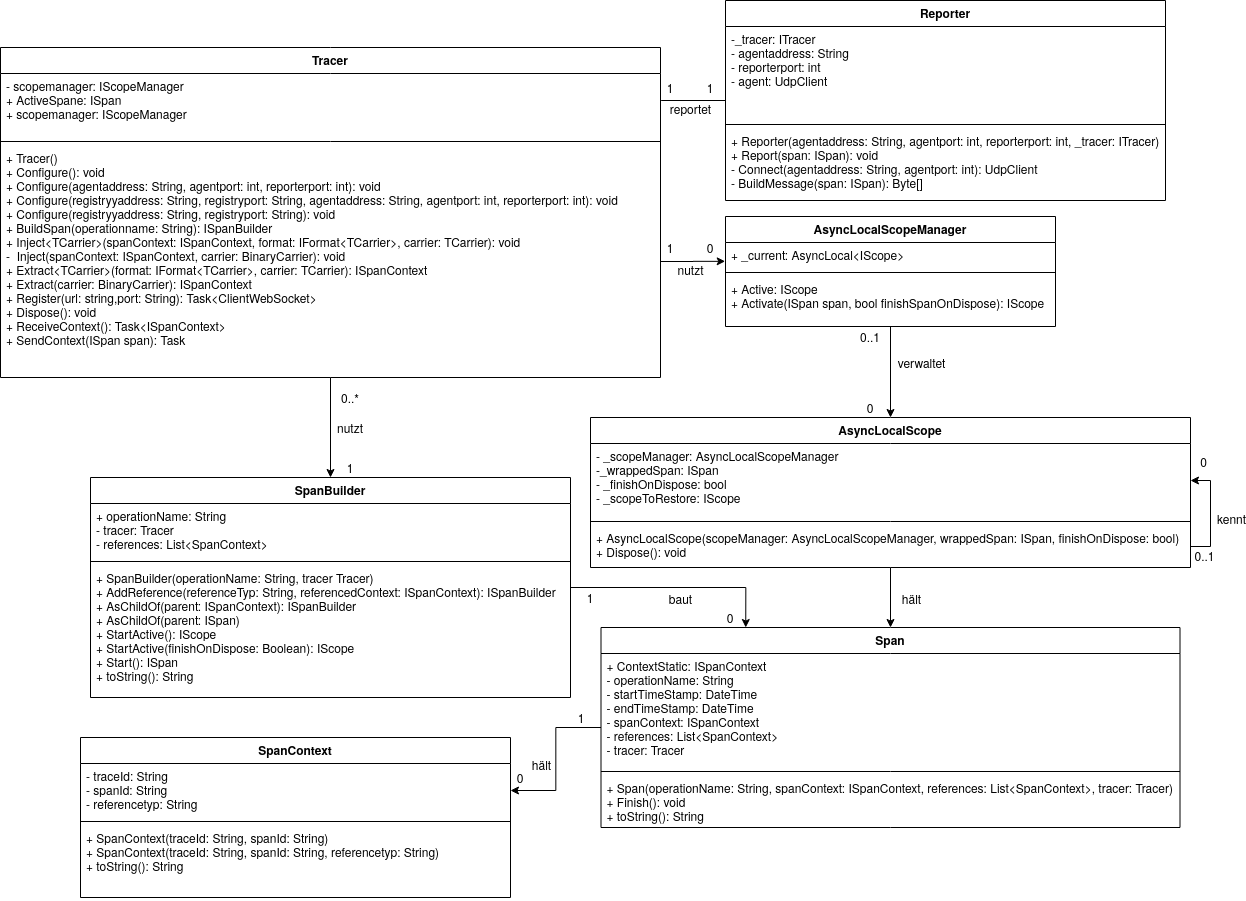
\includegraphics[scale=0.4]{img/Implementierung/TraktorKlassendiagramm.png}
		\caption[Klassendiagramm der Traktor Instrumentalisierungsbibliothek]{Klassendiagramm der Traktor Instrumentalisierungsbibliothek}
		\label{fig:TraktorKlassendiagramm}
	\end{figure}
\end{landscape}

\section{Traktor Agent}
\label{section:Traktor Agent}

Der Traktor Agent ist ein Service, welcher einen \gls{udpLabel}-Endpunkt bereitstellt. Der Service gibt alle erhaltenen Nachrichten auf seiner Konsole aus. Zwei Umgebungsvariablen werden genutzt, um den \gls{udpLabel}-Endpunkt zu initialisieren. Die \textbf{UDP\_IP} ist der \emph{Localhost}, da der Service auf einer eigenständigen Komponenten bereitgestellt wird. Dies ist durch den Spezifikikationspunkt \textbf{TE}.2  gegeben. Der belegete Port wird durch die Umgebungsvariable \textbf{UDP\_PORT} konfiguriert. 

Ein reporteter Span kann folgendermaßen aussehen:

\begin{minipage}[]{\textwidth}
	\begin{lstlisting}[frame=trBL]
	traktor-agent_1| recieved message: 
		 b'Process Context;
		 04/14/2020 10:10:06.1791 PM;
		 WIoJiNwldhLM;ZtDdH4lQ1a1b;
		 child_of;
		 04/14/2020 10:10:06.4158 PM'
	traktor-agent_1| from:  ('172.22.0.5', 13338)
	\end{lstlisting}
	\captionof{lstlisting}{Ein reporteter Span. Der gezeigte Span ist in der Webserver Entwicklungsumgebung generiert worden}
	\label{listing:Reporteter-Span}
\end{minipage} 

Der Service \emph{traktor-agent\_1} erhält von der Netzwerkadresse 172.22.0.5:13338 die dargestellte Nachricht eines Spans mit dem Operationsnamen \emph{Process Context}. Der Startzeitstempel und der Endzeitstempel sind Teil des reporteten Spans. Auch der Spankontext ist dargestellt.

\section{Traktor Registry}
\label{section:Traktor Registry}

Die Traktor Registry ist ein Websocket Server. Verbindungsanfragen, initiiert von einer Tracerinstanz, werden als eigenständiger Thread in einer Klienten-liste der Registry gespeichert. Die Anwendungslogik der \emph{ClientHandler}-Threads implementiert die Websocket Handshakes. Das Websocketprotokoll wird in \cref{subsection:Websocketprotokoll} beschrieben. Die Kontextpropagierung wird durch den Websocket Server umgesetzt. Die Implementierung wird in \cref{subsection:Klientenverwaltung} vorgestellt.

\subsection{Websocketprotokoll}
\label{subsection:Websocketprotokoll}

Das Websocketprotokoll ermöglicht eine voll-duplex Kommunikation zwischen der Registry und dem entsprechenden Websocketklienten eines Tracers. Das Protokoll nutzt dafür eine einzige TCP-Verbindung. Das Websocketprotokoll wird genutzt, um einen geringen \textbf{Overhead} der Kommunikation zu gewährleisten. Dementsprechend wird das Designziel der \textbf{Verarbeitungskosten} berücksichtigt. Das Websocketprotokoll ist durch \gls{rfcLabel} mit der Nummer 6455 spezifiziert.

Das Websocketprotokoll verlangt einen öffnenden Handshake zur Etablierung der Verbindung. Dieser basiert auf einem HTTP Handshake. Die eröffnende HTTP-Anfrage beinhaltet eine \emph{Upgrade}-Anforderung, der in diesem Moment genutzten HTTP-Verbindung. Der folgende Ausschnitt eines Logs, zeigt eine solche Eröffnungsnachricht:

\begin{minipage}[]{\textwidth}
	\begin{lstlisting}[frame=trBL]
	GET / HTTP/1.1
	Host: traktor-registry:8090
	Connection: Upgrade
	Upgrade: websocket
	Sec-WebSocket-Version: 13
	Sec-WebSocket-Key: s4VKefPmikGz1rJ24buoaQ==
	\end{lstlisting}
	\captionof{lstlisting}{Eröffnende Nachricht eines Websocket Handshake}
	\label{listing:Eröffnender Websocket Handshake}
\end{minipage} 

Die HTTP-Nachricht beinhaltet sogenannte \textbf{Header}, die Daten beinhalten, die für den Protokollwechsel von HTTP zu Websocket nötig sind. Der Host-Header identifiziert den Ursprung des Handshakeinitiators. Dieser ist in diesem Falle die IP-Addresse die hinter dem Alias \emph{traktor-registry} steht. Der Port 8090 der Anwendung, von welchem die Anfrage stammt, wird zusätzlich mitgesendet. Der Connection-Header gibt die bevorzugte Verbindungsart an. Diese beschreibt den gewünschten Vorgang eines Upgrades der Verbindung. In Verbindung mit dem Inhalt des Connections-Headers wird ein Upgrade-Header gesendet. Dieser ist ein Vorschlag an den Server ein anderes Protokoll zu nutzen. Entsprechend beinhaltet der Upgrade-Header den Vorschlag das Websocket Protokoll zu verwenden. Die letzen beiden Header Sec-WebSocket-Version und Sec-WebSocket-Key sind websocketspezifische Header.

Die Serverantwort sieht ähnlich aus. Diese besteht aus der Request-Line und dem Sec-WebSocket-Accept Header, der eine Bestätigung der zu nutzenden Websocketverbindung darstellt.

\begin{minipage}[]{\textwidth}
	\begin{lstlisting}[frame=trBL]
	HTTP/1.1 101 Switching Protocols
	Upgrade: websocket
	Connection: Upgrade
	Sec-WebSocket-Accept: HSmrc0sMlYUkAGmm5OPpG2HaGWk=
	\end{lstlisting}
	\captionof{lstlisting}{Serverantwort eines Websocket Handshake}
	\label{listing:Serverantwort eines Websocket Handshake}
\end{minipage} 

Bei einem erfolgreichen Handshake bleibt die Verbindung kommunikationsbereit, bis der Tracer die Verbindung manuell schließt.

Die Implementierung des Websocket Servers basiert auf Grundlage eines Guides von Mozilla und wurde entsprechend den Implementierungsanforderungen angepasst und erweitert.\footpartcite{MozillaWebsocket} Nachfolgend wird die Implementierung der Antwort auf einen Websocketverbindungsanfrage gezeigt:

\begin{minipage}[]{\textwidth}
	\begin{lstlisting}[frame=trBL]
	string swk = Regex.Match(s, "Sec-WebSocket-Key: (.*)")
									.Groups[1].Value.Trim();
	string swka = swk + "258EAFA5-E914-47DA-95CA-C5AB0DC85B11";
	byte[] swkaSha1 = System.Security.Cryptography.SHA1.Create()
									.ComputeHash(Encoding.UTF8
									.GetBytes(swka));
	string swkaSha1Base64 = Convert.ToBase64String(swkaSha1);
	
	byte[] response = Encoding.UTF8.GetBytes(
									"HTTP/1.1 101 Switching Protocols\r\n" +
									"Connection: Upgrade\r\n" +
									"Upgrade: websocket\r\n" +
									"Sec-WebSocket-Accept: " + swkaSha1Base64 +
									"\r\n\r\n");
	
	stream.Write(response, 0, response.Length);
	\end{lstlisting}
	\captionof{lstlisting}{Implementierung der Serverantwort eines Websocket Handshake}
	\label{listing:Implementierung der Serverantwort eines Websocket Handshake}
\end{minipage}

Der Wert von \emph{Sec-WebSocket-Key} wird extrahiert und von führenden und folgenden Leerzeichen bereinigt. Anschließend wird der Wert mit einer speziellen \gls{guidLabel} konkateniert. Dieser zusammengesetzte String wird schließend mit SHA-1\footpartcite{fette2011websocket}, einem kryptographischen Hash Algorithmus, verschlüsselt. Der verschlüsselte Wert wird daraufhin mit Base64 kodiert, die Serverantwort gebaut und anschließend an den Tracerklienten gesendet.

Der Websocket Server muss in der Lage sein, auf eine Schließung der Websocketverbindung reagieren zu können. Dementsprechend muss eine Schließungsnachricht gebaut werden.
Diese Schließungsnachricht ist ein 2-Byte großer Frame. Die \cref{fig:WebsocketClosingFrame} visualisiert einen Websocketschließungs-Frame. Der Frame besteht aus einem FIN-Bit, der auf 1 gesetzt sein muss. RSV1, RSV2 und RSV3 sind reservierte Bits, die auf 0 gesetzt sein müssen. Der Opcode ist ein 4-Bit großer Flag, der dem Dezimalwert 8 entspricht. Dieser steht für die Operation des Schließens des Websockets. Die Maske ist auf 0 gesetzt. Auch sind die Bits der Payload Length auf 0 gesetzt. 

\begin{figure}[!ht]
	\centering
	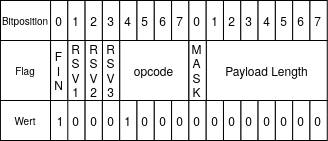
\includegraphics[scale=0.8]{img/Implementierung/WebsocketClosingFrame.png}
	\caption[Websocket Closing Frame]{Websocket Closing Frame}
	\label{fig:WebsocketClosingFrame}
\end{figure}


\subsection{Klientenverwaltung}
\label{subsection:Klientenverwaltung}

Bei erfolgreich hergestellter Websocketverbindung, kann die Registry auf Kontextpropagierung reagieren. 
Die Klienten werden in einem seperaten Thread behandelt. 
Ein Thread beinhaltet jeweils einen Datenstrom. 
Der Thread implementiert eine Dauerschleife. 
In dieser Dauerschleife wird der Datenstrom kontinuierlich überprüft. 
Bei eingehenden Daten wird überprüft, um welchen Datentypen es sich handelt. 
Dieser Prozess ist zum Teil in dem Aktivitätsdiagramm, gezeigt in \cref{fig:Traktor-Registry}, visualisiert.
Es werden drei Nachrichtentypen unterschieden:
\begin{itemize}
	\item Tracerklient Anmeldung
	\item Tracerklient Abmeldung
	\item Kontextübermittlung
\end{itemize}

Der Nachrichtentyp der Anmeldung, lässt sich anhand der Request-Line feststellen. 
Bei Abmeldungen und Nachrichten, die Kontextübermittlung einleiten sollen, kann dies durch den \emph{opcode} festgestellt werden.
Die Implementierungsdetails der An- und Abmeldung wurde in \cref{subsection:Websocketprotokoll} ausgeführt. 
Im Falle der Kontextübermittlung wird die Nachricht zuerst decodiert. 
Da die Nachricht von einem Websocketklienten stammt, ist der \textbf{Mask} bit gesetzt. 
Dies ist in \gls{rfcLabel} 6455 spezifiziert. 
Dementsprechend muss die Nachricht umformatiert werden, damit sie weiterverarbeitet werden kann. Die Nachricht wird im Registry-Log ausgegeben und anschließend wird der Kontext an alle Teilnehmenden Tracerklienten versendet. In der Implementierung ist noch keine Addressierung der Kontextnachrichten umgesetzt. Das bedeutet, dass alle teilnehmenden Klienten die Kontextnachricht empfangen, abgesehen von dem Klienten, der die Nachricht versendet hat. Dies kann in Systemen mit mehr als zwei Tracerinstanzen zu Komplikationen mit dem Nachrichtenstrom führen, da abgesehen von dem Zieltracer des Kontext, keine Kontextnachrichten erwartet werden.

\section{Traktor Interceptor}
\label{section:Traktor Interceptor}
Der Traktor Interceptor dient als Alternativkonzept zu der Traktor Registry. Der Traktor Interceptor setzt eine Nachrichtenmodifikation um, bei der die Nachrichten, die durch die Betriebssystemnetzwerksinterfaces geleitet werden, abgefangen und erweitert werden. Bei dem Eintreffen der Nachricht in der Empfängerkomponente wird die Nachricht abermals abgefangen und die Metadaten extrahiert. Der Traktor Interceptor wird als Python Script umgesetzt. Auf jeder Komponente des Systems muss dieses Script während der Laufzeit der instrumentalisierten Anwendung ausgeführt werden. Der implementierte Prototyp soll als \emph{Proof of Concept} dienen. Das Abhören der Netzwerkschnittstelle und das Manipulieren der Pakete ist mithilfe der Paketmanipulationsbibliothek Scapy umgesetzt. Das Script beinhaltet eine Schleife, bei der bei eintreffender Websocketnachricht eine Callback Funktion aufgerufen wird. Die Callback Funktion erhält als Parameter die Nachricht. Es wird untersucht, ob die Nachricht den Spezifikationen eine Websocketnachricht entspricht. Anschließend wird die Nachricht in ihre Komponenten zerlegt, wieder zusammengebaut und an ihren Empfänger weitergeleitet. Der Prototyp zeigt, dass eine Paketmanipulation möglich ist.

\section{Unity Rendering-System}
\label{section:Unity Rendering System}

Das verteilte Rendering-System dient zur Generierung von Frames auf Grundlage von dreidimensionalen Geodaten. Dabei wird ein Ansatz verwendet, um die Vorteile einer verteilten Anwendung zu nutzen. Das heißt, dass viele Komponenten des Systems Teilaufgaben bearbeiten. Die Arbeit, die von den Komponenten verrichtet wird, ist das Generierung von Teilframes. Die Teilframes werden in einem Kollektor zusammengeführt und anschließend an den anfragenden Klienten gesendet. Die Anwendung verwendet die Unity Engine als Renderer. Die Instrumentalisierung findet innerhalb der Scripts statt, die für den Renderprozess ausgeführt werden. In dem verteilten Rendering-System ist das Event des Generierens und des Absendens eines Frames von Interesse. Dieses Event wird von der Instrumentalisierungsbibliothek als Traces dargestellt.
Dadurch wird die Zeit aufgezeichnet, die für die Generierung eines Frames benötigt wird. Aufgrund der Struktur des Projekts, lassen sich keine detaillierteren Events, wie z.B. das Empfangen der Klientenanfrage oder das Senden des Frames, darstellen. 

Die Instrumentalisierung ist durch das Hinzufügen eines Scripts und der Modifikation eines bestehenden realisiert.
Das hinzugefügte Script \emph{LoggingServerSideRendering} beinhaltet eine Klasse, dessen Objekt als Tracer innerhalb eines Scripts genutzt werden kann.
Aufgrund der hoch asynchronen und parallelen Natur der Appliktion ist es notwendig eine dynamische Portermittlung für den Reporter zu ermöglichen.
Dazu wurde ein Portbereich bekanntgegeben, in dem ein freier Port ausgewählt wird.
Jeder parallele Prozess, der einen Tracer nutzt, wartet auf die Beendigung des Konfigurationsprozesses des Tracers.
Dies hat zur Folge, dass die Prozesse auf den Tracer warten müssen.
Das widerspricht dem Designziel der Verarbeitungskosten. Dieser Umstand ist jedoch als Kompromiss zu sehen. Der Kompromiss besteht darin, die Nutzung des Tracers innerhalb der Unity Anwendung möglichst benutzerfreundlich zu machen, also dem Designziel der Benutzbarkeit zu entsprechen.

Die Instrumentalisierung befindet sich in der \emph{GBufferSource} Klasse.
Die Klasse umfasst den Renderingvorgang eines Frames. 
Dieser Vorgang wird als ein zu verfolgendes Event bestimmt.
In \cref{listing:Instrumentalisierung der GBufferSource Klasse} ist der Codeabschnitt dargestellt, der instrumentalisiert ist.
Die Instrumentalisierung umfasst das Rendern, durchgeführt durch ein \emph{\_camera} Objekt und die Frameextraktions aus dem nativen Plugin.


\begin{minipage}[]{\textwidth}
	\begin{lstlisting}[frame=trBL]
	using (var scope = LoggingServerSideRendering.Tracer
					.BuildSpan("Render Frame")
					.StartActive(true))
	{
				_camera.Render();
				_nativeGBufferExtraction.NewFrameRendered(Time.frameCount);
	}
	
	\end{lstlisting}
	\captionof{lstlisting}{Instrumentalisierung der GBufferSource Klasse}
	\label{listing:Instrumentalisierung der GBufferSource Klasse}
\end{minipage}

\section{ Webserver Entwicklungsumgebung }
\label{section:Webserver Entwicklungsumgebung}

In diesem Kapitel wird die Traktorentwicklungsumgebung vorgestellt. Diese Testumgebung gewährleistet, dass die Funktionalitäten der Instrumentalisierungsbibliothek in einer Beispielanwendung angewandt werden können. Das System besteht aus vier Komponenten. Eine Übersicht der Komponenten ist in der \cref{fig:TraktorEnv-ApplicationArchitecture} gezeigt. Neben der bereits beschriebenen Traktor Registry und dem Traktor Agent, werden zwei Webserver eingeführt. Die beiden C\# Webserver \emph{Traktor-Fibonacci-Caller} und \emph{Traktor-Fibonacci-Server} sind mit Traktor instrumentalisiert. Sie dienen dazu, einen Nachrichtenaustausch zu ermöglichen, der sich durch das ganze System zieht. Die Applikation ermöglicht es einem Anwender, eine Zahl der Fibonacci-Folge zu berechnen. Die Nachricht die der Anwender an den Traktor-Fibonacci-Caller-Service sendet, beinhaltet im \emph{Body} eine Zahl mit dem Variablennamen N. Die Zahl repräsentiert die zu berechnende Stelle der Fibonacci-Folge. In \cref{listing:Implementierung der Serverantwort eines Websocket Handshake} wird eine beispielhafte Anfrage gezeigt. Es wurde sich für die Implementierung eines simplen und rekursiv anwendbaren Algorithmus entschieden, da die Testumgebung nicht durch die Anwendungslogik der Webserver verkompliziert werden sollte. Ausserdem ermöglich die Rekursivität des Algorithmus, eine schnell zu skalierende Anzahl an generierten Events, mit einem deutlich erkennbaren und messbaren zeitlichen Unterschied. Die Grundstruktur der beiden Webserverimplemetierungen ist gleich. Ein C\# Programm startet ein Serverobjekt, welcher einen Thread beinhaltet, der eine API bereitstellt, die über HTTP ansprechbar ist. Nachfolgend wird auf die Instrumentalisierung der Webserver eingegangen.

\begin{minipage}[]{\textwidth}
	\begin{lstlisting}[frame=trBL]
	PUT / HTTP/1.1
	Accept: application/json, */*
	Accept-Encoding: gzip, deflate
	Connection: keep-alive
	Content-Length: 8
	Content-Type: application/json
	Host: 172.22.0.5:8085
	User-Agent: HTTPie/0.9.8
	
	{
	"N": 3
	}
	\end{lstlisting}
	\captionof{lstlisting}{HTTP-Anfrage an den Traktor-Fibonacci-Caller durch den HTTP-Klient HTTPie}
	\label{listing:Implementierung der Serverantwort eines Websocket Handshake}
\end{minipage}


\textbf{Traktor-Fibonacci-Caller}\space\space\space Sowohl der Traktor-Fibonacci-Caller als auch der Traktor-Fibonacci-Server basieren auf dem gleichen Aufbau. Beim Starten der Anwendung wird, abhängig von der Betriebssystemfamilie, die Tracerkonfiguration durchgeführt. 
Auf einem Unix-basierenden Betriebssystem, wird die Konfiguration über Umgebungsvariablen gehandhabt. 
Da der Server einen Tracer beinhaltet, sind die für die Registry-Verbindung benötigten Umgebungsvariablen zu setzten. 
Diese sind die \emph{REGISTRY\_IP} und der \emph{REGISTRY\_PORT}. 
Für die Verbindung zum Traktor-Agenten werden die entsprechenden Umgebungsvariablen \emph{AGENT\_IP} und \emph{AGENT\_PORT} erwartet.
Für den einzunehmenden Port des Tracers, über den die reporteten Spans zum Agenten gesendet werden, wird der \emph{REPORTER\_PORT} zur Konfiguration genutzt. 
Der Server ist nach seiner Initialisierung einsatzbereit und erwartet Nachrichten. 
Sobald eine Nachricht eintrifft, wird die \emph{Proccess} Funktion aufgerufen. 
Die Process Funktion erhält einen HTTP Kontext als Paramenter. 
Dieser beinhaltet die Nutzdaten des Anwenders, die mittels HTTP-Klienten gesendet wurden.

Der instrumentalisierte Codeabschnitt des Callers ist folgendermaßen implementiert:

\begin{minipage}[]{\textwidth}
	\begin{lstlisting}[frame=trBL]
	private void Process(HttpListenerContext context){
		using (var scope = Program.tracer.BuildSpan("Process Context")
						.StartActive())
		{
			var body = new StreamReader(context.Request.InputStream, Encoding.UTF8)
						.ReadToEnd();       
			var json = JsonSerializer.Deserialize<JsonObject>(body);
			Program.tracer.SendContext(scope.Span).GetAwaiter().GetResult();
			string response = SendRequest(fibo_ip,fibo_port,json);
			context = BuildResponse(context, response);
			context.Response.Close();
		}
	}
	\end{lstlisting}
	\captionof{lstlisting}{Process Funktion des Fibonacci-Caller Services}
	\label{listing:Process Funktion des Fibonacci-Caller Services}
\end{minipage}

Das \emph{using} Statement dient zum automatischen Schließen, der in ihr genutzten Ressource. 
Dies ist in diesem Fall das Scope Objekt. 
Der Tracer baut einen neuen Span mit dem Operationsnamen \emph{Process Context} und makiert in als aktiv. 
Die Nutzdaten werden aus der HTTP-Nachricht extrahiert. 
Die aktuell als JSON-Objekt vorliegenden Daten, werden deserialisiert. 
Da der Tracerkontextwechsel bevorsteht, wird der Kontext des Spans an die Registry, mittels \emph{SendContext}, gesendet und auf einen erfolgreichen Abschluss gewartet. 
Es ist zu diesem Zeitpunkt davon auszugehen, dass der Zieltracer bereit ist, den empfangen Kontext zu verarbeiten. 
Aus diesem Grund werden die Nutzdaten an den Trakor-Fibonacci-Server im JSON-Format als weiterer Request gesendet. 
Sobald das Ergebnis vom Fibonacci Server eintrifft, wird die Antwort, welcher zum HTTP-Klienten zurückkehrt, gebaut und übermittelt. 
Aufgrund des using-Statements beendet die Lebensspanne des Scope Objekts und der Span wird an den Traktor-Agent reportet. 

\textbf{Traktor-Fibonacci-Server}\space\space\space Der Fibonacci-Server beinhaltet den Algorithmus zur Berechnung der Fibonaccizahl. 
Innerhalb des Server sind zwei Funktionen instrumentalisiert. Dies ist zum einen, wie auch im Fibonacci-Caller, die \emph{Process} Funktion, aufgeführt in \cref{listing:Process Funktion des Fibonacci-Server Services}. 
Die Funktion zeigt das Empfangen des Tracingkontexts durch den Aufruf der Funktion \emph{ReceiveContext}. Ein neuer Span wird manuell erstellt. 
Die Relation wird durch die Tracerfunktionalität \emph{AsChildOf(parentContext)} hergestellt. 
Anschließend wird der Span gestartet und aktiviert. 
Die Nutzdaten werden extrahiert und die zweite instrumentalisierte Funktion \emph{CalculateFibonacci} wird aufgerufen. 

\begin{minipage}[]{\textwidth}
	\begin{lstlisting}[frame=trBL]
	private async void Process(HttpListenerContext context)
	{
		ISpanContext parentContext = await Program.tracer
							.ReceiveContext();
		string response;
		var span = Program.tracer.BuildSpan("Server: Process Context")
							.AsChildOf(parentContext)
							.Start();
		Program.tracer.ScopeManager.Activate(span,true);
		var body = new StreamReader(context.Request.InputStream, Encoding.UTF8)
							.ReadToEnd();       
		var json = JsonSerializer.Deserialize<JsonObject>(body);
		response = CalculateFiboncacci(json.N).ToString();
		response = "result=" + response;
		byte[] b = Encoding.UTF8.GetBytes(response);
		[...]
		context.Response.Close();
		span.Finish();
	}
	\end{lstlisting}
	\captionof{lstlisting}{Process Funktion des Fibonacci-Server Services}
	\label{listing:Process Funktion des Fibonacci-Server Services}
\end{minipage}

Die CalculateFibonacci Funktion ist bewusst rekursiv und möglichst ineffizient implementiert. Die Funktion braucht zur Berechnung des $n$te Elements $(2 * Fn) - 1$ rekursive Aufrufe, wobei $Fn$ die ermittelte Fibonaccizahl ist. Dadurch ist es möglich, einen großen Trace zu erzeugen. Die Funktion nutzt das using-Statement, um beim Beenden des Codeabschnitt den Span automatisch zu reporten. \emph{CalculateFibonacci} ist als Operationsname gegeben.

\begin{minipage}[]{\textwidth}
	\begin{lstlisting}[frame=trBL]
	private int CalculateFiboncacci(int n) 
	{
		using (var scope = Program.tracer.BuildSpan("CalculateFiboncacci")
						.StartActive())
		{
			if (n == 0) return 0;
			else if (n == 1) return 1;
			return  ( CalculateFiboncacci(n - 1) + CalculateFiboncacci(n - 2) );
		}
	}
	\end{lstlisting}
	\captionof{lstlisting}{Instrumentalisierte CalculateFibonacci Funktion des Fibonacci-Server Services}
	\label{listing:Instrumentalisierte CalculateFibonacci Funktion des Fibonacci-Server Services}
\end{minipage}

\cref{fig:TraktorEnv-ApplicationArchitecture} bietet eine Architekturübersicht. Es werden die Kommunikationswege, sowie die Services dargestellt, die implementiert und beschrieben wurden.

\begin{figure}[]
	\centering
	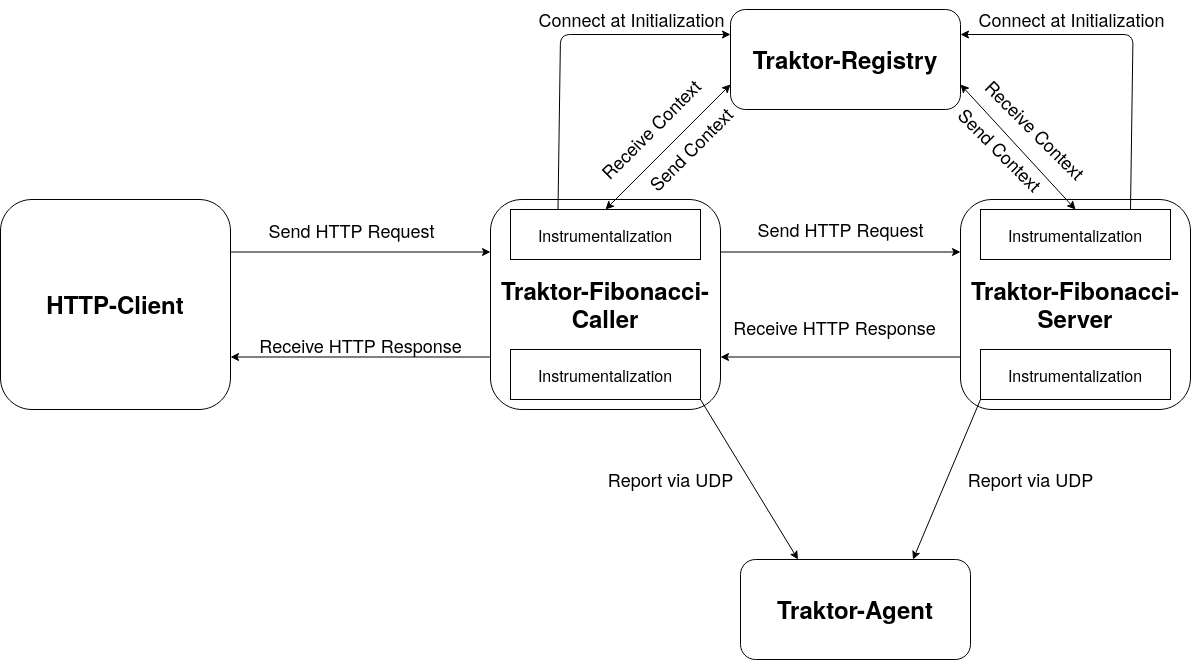
\includegraphics[scale=0.3]{img/Implementierung/TraktorEnv-ApplicationArchitecture.png}
	\caption[Systemübersicht der Traktorentwicklungsumgebung]{Systemübersicht der Traktorentwicklungsumgebung}
	\label{fig:TraktorEnv-ApplicationArchitecture}
\end{figure}
% ----------------------------------------------------------------------------
